\section{Další nastavení}
%%%%%%%%%%%%%%%%%%%%%%%%%%%%
Pro splnění požadavku na českou lokalizaci je potřeba provést nastavení jazyka. Vyplnění informací o organizaci je spíše formalitou.
%%%%%%%%%%%%%%%%%%%%%%%%%%%%
\subsection{Česká lokalizace}
Česká lokalizace systému proběhla skrze záložky \emph{Language Settings}, kde byla do systému přidána čeština. 

Dalším krokem byl překlad atributů objektů z anglického jazyka do češtiny. Tento překlad je dostupný v menu \emph{Translation Workbench -- Translate}, kde po výběru objektu je možné atributy překládat. Rozhraní překladu je vidět na obrázku \ref{fig:Translation}.

Překlad objektů není v současné době k dispozici. Alternativou je přejmenování záložek, které je dostupné v menu \emph{Rename Tabs and Labels}. Nevýhodou tohoto přejmenování je, že vede k přejmenování záložek ve všech systémových jazycích. Toto přejmenování bylo provedeno do češtiny.

Jazyk rozhraní si potom vybírá uživatel sám, v nastavení svého profilu.

\begin{figure}[h!]
    \centering
    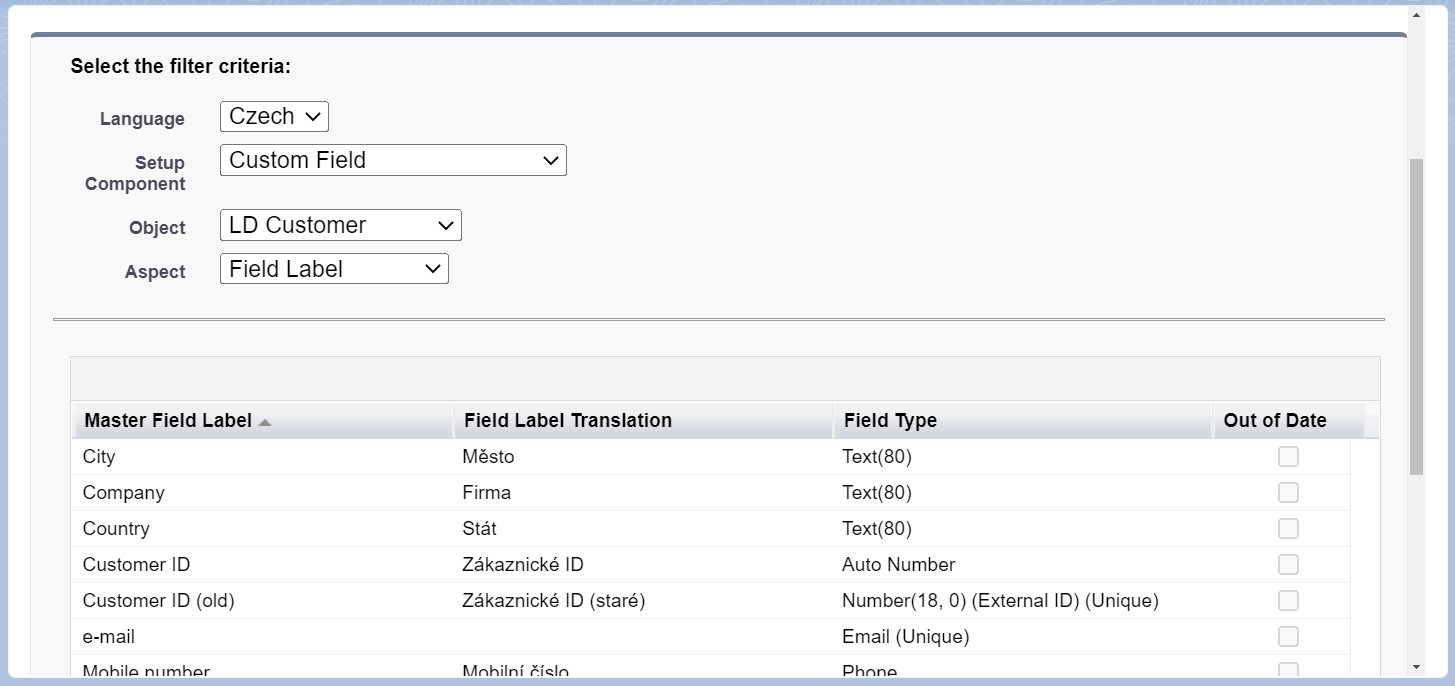
\includegraphics[width=\textwidth]{assets/7_implementace/finální_nastavení/překlad.png}
    \caption{Rozhraní překladu.}
    \label{fig:Translation}
\end{figure}
\FloatBarrier

\subsection{Informace o oragnizaci}
V menu \emph{Company Settings} byly vyplněny základní informace o organizaci, jako pracovní doba, adresa nebo výchozí měna.